\chapter{Routing}

Routing determine the ``good''\footnote{The minimum path typically} path (
sequence of routers) thru network from source to destination.
Routing protocols use graphs as a mathematical abstraction.

\section{Typologies of routing}

Routing can be \textbf{global}, \textbf{decentralized}, \textbf{static} (where
the route change slowly over time) and \textbf{dynamic} (where the routes change
quickly over time).

\subsection{Global routing}

In this kind of routing routers have the complete topology of the network, with
information about links cost.
Characteristics:
\begin{itemize}
\item ``link state'' algorithm
\item efficent but not faseable
\end{itemize}

An example of a global routing algorithm is the one made by Dijkstra.

\subsubsection{Dijkstra's algorithm}

In this algorithm, that's iterative, all the nodes know link cost between each
other. Basically, it computes least cost path from one note to all the others.

\begin{figure}[t]
  \captionsetup{singlelinecheck=off}
  \centering
  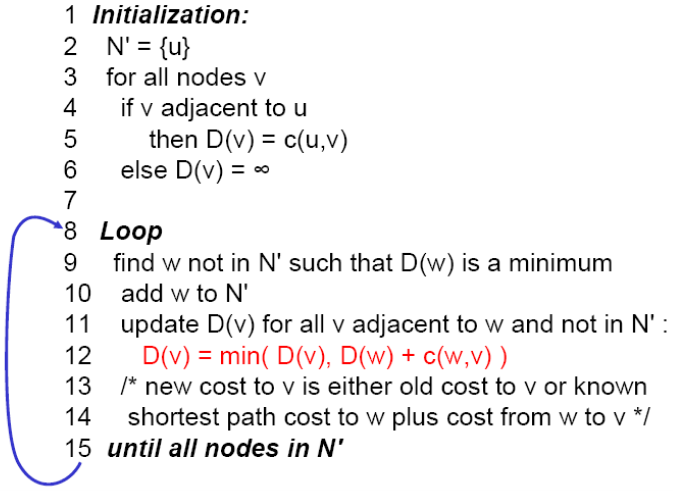
\includegraphics[scale=0.45]{DijkstraAlgo}
  \caption[Dijkstra's algorithm]{Dijkstra's algorithm. Notation:
    \begin{itemize}
    \item $c(x, y)$: link cost from node $x$ to $y$. It's $\infty$ if not direct
      neighbors
    \item $D(v)$: current value of cost of path from source to destination $v$
    \item $p(v)$: predecessor node along path from source to $v$
    \item $N'$: set of nodes whose least cost path definitively known
    \end{itemize}
  }
\end{figure}

\subsection{Decentralized routing}
In this type of routing routers know physically-connected neighbors, and link
cost to them. There is a iterative process of computation and exchange of
information with neighbors.
This algorithms are defined as ``distance vector'' algorithms.

\subsection{Routing based on network typology}

There are different types of routing based on different types of networks.

\paragraph*{Infrastructure based} In this case routing is relatively simple.
There is just a simgle hop from the access point (AP) to the wireless node.

\paragraph*{MANET} Also know as ad-hoc, it has the following characteristics:
\begin{itemize}
\item the network costantly changes
\item wireless nodes are not necessarily all adjacent, so data forwarding
  could be necessary
\end{itemize}
Additionally, there are other difficulties, such as energy consumption and
limited bandwidth (due exchange of routing information) on mobile systems. In
wireline networks we have symmetric links, limited redundancy and fixed
typology, insteas in wireless has asymmetric links, random redundancy with
unplanned, dynamic links. With all this pecurialities, traditional routing
algorithms for MANETS\footnote{MANET stands for \textit{Metropolitan Area
    Network}} are inefficent, and the new one must rely on data link
information, not just network layer updates\footnote{Layer updates only
  determine connectivity}, without using in centralized approaches because they
just don't work. In MANETS nodes can be routers, and they can send different
type of messages between them.
\subparagraph*{Messages classification} There are different type of messages:
\begin{itemize}
\item Unicast: trasmission 1 to 1. In order to achieve a good unicast routing
  protocol there are some goals:
  \begin{itemize}
  \item minimal control overhead
  \item multi-hop path routing capability
  \item no loops
  \end{itemize}
\item Multicast: transmission 1 to N: different receivers of the same message,
  that it can follow different paths
\item Broadcast: transmission 1 to N: everyone receives the message
\end{itemize}

\section{Protocols classification}

Protocols can be proactive or reactive, and are classificated as:
\begin{itemize}
\item table-driven (proactive) $\to$ up-to-date routing information are
  maintained
\item source-initiated (on demand/demand driven) $\to$ only routes in use are
  maintained
\item hybrid protocols $\to$ combination of proactive and reactive protocols
\end{itemize}

\subsection{Proactive protocols}

Proactive protocols are based on traditional distance-vector and link-state
protocols, where each node maintains a route to the other edge of the network.
This cause a high overhead in most scenarios, but since each node maintains and
updates its routing table, there is a low packet forwarding latency.

Due the proactive nature, changes to the network topology are immediately
propagated to all the nodes.

There are different typologies, that will be described below.

\subsubsection{DSDV (Destination Sequenced Distance Vector)}

Based on Bellum-Ford algorithm it has characteristics similar to Dijkstra's
algorithm, but with slower performace and a better versatility (it supports
negative weights). With DSDV, every route has a sequence number and packets are
transmitted according to the routing table: each node has a routing table with
all the nodes listed, and each node has its own sequence number.
The routing table consistency is kept trasmitting periodically updates and when
two routes to a destination is received from two different neightbors the one
with the gratest destination dequence number is choosen, otherwise the smallest
leap-count is kept % TODO check this part
Continuously updating the routing table can generate a lot of overhead, and
there are two ways to carry updates:
\begin{itemize}
\item performing a full dump
\item having incremental updates
\end{itemize}

\subsubsection{OLSR (optimized link state routing)}

This is based on the link state algorithm. It minimizes flooding of broadcasting
packets by using only the selected \textit{Multipoint Hop (MH)} called
\textit{Multipoint relays (MR)}. All links with neighboring MHs are declared and
are flooded in the entire network. MR minimize the flooding by reducing
duplicate retrasmission.

In general, OLSR is good for large and dense networks.

\subsubsection{CGSR}

In this typology, nodes are organized into a hierarchy of clusters: every
cluster has a \textit{cluster master (clusterhead)} that forward packets from
the other sets node.

\subsection{Reactive protocols}
